% This file was converted to LaTeX by Writer2LaTeX ver. 1.2
% see http://writer2latex.sourceforge.net for more info
\documentclass[11pt]{article}
\usepackage[utf8]{inputenc}
\usepackage[T1]{fontenc}
\usepackage[spanish,english]{babel}
\usepackage{amsmath}
\usepackage{amssymb,amsfonts,textcomp}
\usepackage{array}
\usepackage{supertabular}
\usepackage{hhline}
\usepackage{graphicx}
\makeatletter
\newcommand\arraybslash{\let\\\@arraycr}
\makeatother
\setlength\tabcolsep{1mm}
\renewcommand\arraystretch{1.3}
\newcounter{Figura}
\renewcommand\theFigura{\arabic{Figura}}
\title{}
\begin{document}
  
   \begin{titlepage}

\begin{center}
\vspace*{-1in}

FACULTAD DE INGENIERIA\\
\vspace*{0.15in}
UNIVERSIDAD DE LA REPUBLICA \\
\vspace*{0.6in}
\vspace*{0.2in}
\begin{Large}
\textbf{Análisis} \\
\end{Large}
\vspace*{0.3in}
\end{center}

\begin{minipage}{0.4\textwidth}
\begin{flushleft} \large
\emph{Autor:}\\
Julio Saráchaga\\
\bigskip
\emph{Contraparte del cliente:}\\
Ing. Fernanda Molina
\end{flushleft}
\end{minipage}
\begin{minipage}{0.4\textwidth}
\begin{flushright} \large
\emph{Supervisor:} \\
Dr. Gustavo Betarte\\
\bigskip
\emph{Supervisor alterno:} \\
Ing. Marcelo Rodríguez
\end{flushright}
\end{minipage}\\[3cm]

\end{titlepage}
  
\clearpage\setcounter{page}{1}\section[Introducción]{Introducción}
Este documento pretende presentar el fundamento de porque utilizar las herramientas seleccionadas, los requerimientos que se identificaron junto con los casos de uso necesarios para resolver dichos requerimientos.

El objetivo de la herramienta es permitir compartir información con socios de confianza para permitir la identificación precisa de amenazas. Por medio de dicha colaboración se permite tener evidencias especificas que den indicios de una entidad maliciosa afectando la organización y que además ayuden a mitigar o erradicar el problema.
Esta herramienta permitiría un intercambio mas eficaz del que existe hoy en día dado que agilizaría los tiempos necesarios para el intercambio por ser automático y estándar.
\section[Porque utilizar TAXII y STIX?]{Porque utilizar TAXII y STIX?}

\bigskip

El lenguaje STIX nos provee una representación estructurada de información de cyber inteligencia que es más expresiva que las utilizadas en la actualidad, consta de una mayor flexibilidad y extensibilidad. La representación de la información utilizada permite el uso de herramientas de automatización sin perder la posibilidad de que la información sea leíble.

STIX facilita el intercambio de información entre organizaciones, comunidades y productos o servicios. Dicho intercambio se realiza por medio de TAXII, este define un conjunto de servicios y mensajes que permiten el intercambio de información entre organizaciones. El intercambio realizado con TAXII permite la detección, prevención y mitigación de amenazas.


\bigskip

También es importante destacar que STIX facilita la descripción y extensibilidad de evidencia y se integra con otras iniciativas de MITRE como lo son MAEC y CAPEC. MITRE ha logrado integrar en STIX estas especificaciones en lugar de re inventor estos componentes. En STIX también se integran otros lenguajes comúnmente utilizados en la comunidad y que tienen propósitos similares como lo es OpenIOC.


\bigskip

Como STIX es un lenguaje XML hereda ciertas propiedades de estos, es un lenguaje extensible, simple y fácil de procesar. 


\bigskip

Además el lenguaje STIX provee expresividad y flexibilidad para expresar \ intrusiones, técnicas utilizadas por los adversarios, identificación de estos entre otras características.


\bigskip

\section[Porque utilizar RTIR?]{Porque utilizar RTIR?}
RTIR es un sistema de manejo de incidentes diseñado para ser utilizado por CERTs y CSIRTs para manejar el creciente número de incidentes reportados. Si bien existen otras herramientas similares, RTIR presenta la ventaja de ser opensource, contar con una API que permite extender la herramienta de forma sencilla. RTIR cuenta además con una comunidad de usuarios grande cuya característica principal es el nivel de estos.


\bigskip

El interés de usar una herramienta de este tipo es la facilidad con la que se manejan los incidentes por medio de ella. Además al ser una herramienta con una profunda inserción en la comunidad, es esperable que sea mas fácil la aceptación de una extensión basada en TAXII y STIX que la creación de una nueva herramienta a la que los usuarios deberán adaptarse.


\bigskip

\section[Selección del modelo]{Selección del modelo}

\bigskip

Durante el relevamiento de requerimientos se decidió que el modelo a implementar seria el Peer To Peer, esto se debe a las características y posicionamiento que desea tener la organización respecto a otros CSIRTs. Otro factor que afecta dicha decisión es la capacidad que tiene la organización de generar y consumir información.

\section[Análisis de requerimientos]{Análisis de requerimientos}
La herramienta que se desea desarrollar busca integrarse con RTIR para realizar un seguimiento de incidentes de seguridad. Esta herramienta debe permitir el intercambio de indicadores entre dos organizaciones, dicho intercambio se realiza por medio de TAXII y la información se codifica utilizando STIX. 


\bigskip

La herramienta debería dar la posibilidad de interactuar por medio del RTIR con otro CSIRT. \ En dicha interacción se podría realizar el manejo de incidentes intercambiando información referente a estos entre los CSIRTs. En dichos intercambios se podría dar información sobre la identificación, solución, atacantes que participaron en el incidente, etc. De esta manera se permite expresar de una mejor forma los incidentes identificados. Cabe recordar que dichos intercambios hoy en día se dan principalmente por medio de foros, mail o comunicaciones telefónicas. Se puede ver que la creación de una herramienta de estas características permitiría una manejo centralizado de la información facilitando el trabajo de los analistas en las distintas organizaciones.


\bigskip

Debe existir la posibilidad de que un analista ingrese nueva información sobre un incidentes al sistema. Luego dicha información debe ser compartida con otra organización. El ingreso de nueva información sobre incidentes puede ser realizada desde el RTIR y luego se debe realizar el intercambio por medio de TAXII. 
Dicha información se representará como un cyber observable en el sistema utilizando STIX.


\bigskip

A pesar de que existe una integración con RTIR, se desea mantener una base de datos separada para el cliente TAXII. Dicha base de datos debe tener la posibilidad de representar objetos STIX y Cybox que sean intercambiados por el cliente TAXII. Esto es deseable para tener la posibilidad de realizar un mejor análisis de la información intercambiada.


\bigskip

Si bien se cuenta con información en bases de datos separadas debe ser posible realizar un mapeo entre incidentes del RTIR e información que este almacenada en la base de datos del cliente TAXII. Seria de interés poder ver cierta información almacenada en la base de datos de TAXII en el RTIR.


\bigskip

Se debe tener la posibilidad de que la herramienta pueda ser extendida. Dando la posibilidad a definir nuevos módulos en el futuro que agreguen funcionalidades al sistema.


\bigskip

Uno de estos módulos que se podría agregar y que es deseado que exista desde la concepción del sistema debe permitir la sanitizacion de la información. Dicha sanitizacion debe alimentarse de políticas definidas por la organización. El módulo debe realizar un análisis de la información previo al intercambio el cual filtre datos sensibles contenidos en los datos a intercambiar. Luego de dicho análisis la información se puede intercambiar entre las organizaciones.


\bigskip

Otro módulo que se desearía agregar es uno de correlación de cyber observables, este debe poder identificar objetos que representen la misma problemática y agruparlos de forma adecuada.


\bigskip

De lo anterior podemos resumir en los siguientes requerimientos funcionales:

\begin{flushleft}
\tablefirsthead{}
\tablehead{}
\tabletail{}
\tablelasttail{}
\begin{supertabular}{|m{5.83516in}|}
\hline
\centering\arraybslash Requerimientos funcionales\\\hline
\begin{itemize}
\item Agregar políticas de sanitizacion de información.
\item Aplicación de las políticas de sanitizacion para la información intercambiada
\item Realizar el intercambio de información de seguridad representada con STIX.
\item Tener la posibilidad de crear información de incidentes de seguridad en el sistema.
\item Realizar un seguimiento y manejo de incidentes de seguridad.
\item La herramienta debe implementar un modelo peer-to-peer de intercambio de información.
\item Se desea poder interactuar con otro CSIRT por medio del RTIR.
\item Tener un módulo de correlación de cyber observables.
\end{itemize}
\\\hline
\end{supertabular}
\end{flushleft}

También se identificaron los siguientes requerimientos no funcionales:


\begin{flushleft}
\tablefirsthead{}
\tablehead{}
\tabletail{}
\tablelasttail{}
\begin{supertabular}{|m{5.83516in}|}
\hline
\centering\arraybslash Requerimientos no funcionales\\\hline
\begin{itemize}
\item Extensibilidad: Debe ser posible extender la herramienta con nuevos módulos que implementen nuevas funcionalidades. Un ejemplo de esto es un modulo de correlación de cyber observables.
\item La herramienta debe mantener la información intercambiada en una base de datos independiente a la de RTIR. Dicha base de datos debe poder representar objetos STIX intercambiados.
\end{itemize}
\\\hline
\end{supertabular}
\end{flushleft}

\bigskip


\bigskip
\newpage

\section[Actores y Casos de Uso]{Actores y Casos de Uso}
\subsection[Actores]{Actores}

\bigskip

\begin{flushleft}
\tablefirsthead{}
\tablehead{}
\tabletail{}
\tablelasttail{}
\begin{supertabular}{m{0.8608598in}m{4.89486in}}
Actor &
Analista\\\hline
\multicolumn{1}{m{0.8608598in}|}{Descripción} &
\multicolumn{1}{m{4.89486in}|}{Este actor tiene la posibilidad de ingresar nueva información en el sistema. Dicha información puede ser intercambiada con otro sistema. Con la información que se ha intercambiado el actor puede realizar un análisis de ella y hacer un manejo de los casos creados en el RTIR.}\\
\end{supertabular}
\end{flushleft}

\bigskip


\begin{flushleft}
\tablefirsthead{}
\tablehead{}
\tabletail{}
\tablelasttail{}
\begin{supertabular}{m{0.8816598in}m{4.8740597in}}
Actor &
Cliente TAXII\\\hline
\multicolumn{1}{m{0.8816598in}|}{Descripción} &
\multicolumn{1}{m{4.8740597in}|}{Este actor es el que interactúa con el sistema para intercambiar datos por medio del protocolo TAXII. El sistema tiene que dar soporte para dicho protocolo para que el intercambio sea exitoso.}\\
\end{supertabular}
\end{flushleft}

\subsection[Casos de uso]{Casos de uso}

\bigskip

\begin{flushleft}
\tablefirsthead{}
\tablehead{}
\tabletail{}
\tablelasttail{}
\begin{supertabular}{m{0.8816598in}|m{4.8740597in}|}
\multicolumn{1}{m{0.8816598in}}{Nombre} &
\multicolumn{1}{m{4.8740597in}}{Ingreso información}\\\hline
Actor &
Analista\\
Descripción &
Este caso de uso comienza cuando el analista desde registrar nueva información en el sistema. Para ello debe ingresar la información que desea ingresar al sistema. Entre la información que puede desear ingresar se encuentran IPs, hash de archivos, descripciones de amenazas, etc. El manejo podría realizarse por medio de los incidentes de RTIR.\\\hhline{~-}
\end{supertabular}
\end{flushleft}

\bigskip

\begin{flushleft}
\tablefirsthead{}
\tablehead{}
\tabletail{}
\tablelasttail{}
\begin{supertabular}{m{0.8816598in}|m{4.8740597in}|}
\multicolumn{1}{m{0.8816598in}}{Nombre} &
\multicolumn{1}{m{4.8740597in}}{Subscripción a TAXII Data Feed}\\\hline
Actor &
Analista\\
Descripción &
Con este caso de uso un analista selecciona un data feed en otro sistema al que quiere subscribirse. Esto se realiza por medio del Feed Managment Service de los sistemas.\\\hhline{~-}
\end{supertabular}
\end{flushleft}

\bigskip

\begin{flushleft}
\tablefirsthead{}
\tablehead{}
\tabletail{}
\tablelasttail{}
\begin{supertabular}{m{0.8816598in}|m{4.8740597in}|}
\multicolumn{1}{m{0.8816598in}}{Nombre} &
\multicolumn{1}{m{4.8740597in}}{Recepción de información}\\\hline
Actor &
Cliente TAXII\\
Descripción &
Este caso de uso se da cuando un cliente TAXII desea enviarle información a nuestro sistema. El envío de información se realiza porque un analista se subscribió a un data feed en el cliente. La recepción de información se realiza por medio del Inbox Service de nuestro sistema.\\\hhline{~-}
\end{supertabular}
\end{flushleft}

\bigskip


\bigskip

\begin{flushleft}
\tablefirsthead{}
\tablehead{}
\tabletail{}
\tablelasttail{}
\begin{supertabular}{m{0.8816598in}|m{4.8740597in}|}
\multicolumn{1}{m{0.8816598in}}{Nombre} &
\multicolumn{1}{m{4.8740597in}}{Envío de información}\\\hline
Actor &
Cliente TAXII\\
Descripción &
Este caso de uso se da cuando el sistema desea enviar información a otro cliente TAXII. El envió de información se realiza porque el cliente se subscribió al TAXII Data Feed del sistema. Esto se realiza por medio del Inbox Service del cliente. El intercambio es iniciado por el sistema.\\\hhline{~-}
\end{supertabular}
\end{flushleft}

\begin{flushleft}
\tablefirsthead{}
\tablehead{}
\tabletail{}
\tablelasttail{}
\begin{supertabular}{m{0.8816598in}|m{4.8740597in}|}
\multicolumn{1}{m{0.8816598in}}{Nombre} &
\multicolumn{1}{m{4.8740597in}}{Poll de información}\\\hline
Actor &
Cliente TAXII\\
Descripción &
Este caso de uso se da cuando un cliente desea recibir información del sistema en un intercambio iniciado por él. Este intercambio se realiza por medio del Polling Service del sistema.\\\hhline{~-}
\end{supertabular}
\end{flushleft}

\bigskip

\begin{flushleft}
\tablefirsthead{}
\tablehead{}
\tabletail{}
\tablelasttail{}
\begin{supertabular}{m{0.8816598in}|m{4.8740597in}|}
\multicolumn{1}{m{0.8816598in}}{Nombre} &
\multicolumn{1}{m{4.8740597in}}{Poll de información a un cliente TAXII}\\\hline
Actor &
Cliente TAXII\\
Descripción &
Este caso de uso se da cuando el sistema desea recibir información de un cliente TAXII en un intercambio iniciado por él. Este intercambio se realiza por medio del Polling Service del sistema.\\\hhline{~-}
\end{supertabular}
\end{flushleft}

\bigskip

\section[Comportamiento de casos de uso]{Comportamiento de casos de uso}

\bigskip

\subsection[Diagrama de casos de uso]{Diagrama de casos de uso}
En el siguiente diagrama se ve en resumen los actores y casos de uso del sistema

\begin{figure}[h]
  \centering
    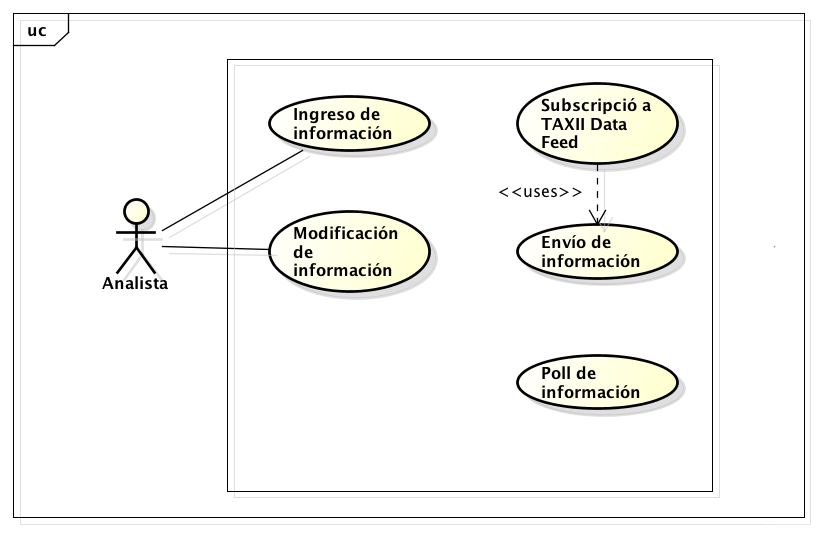
\includegraphics[width=5.7638in,height=3.9299in]{Analisisdelproblema-img/Analisisdelproblema-img006.png}

    Figura \stepcounter{Figura}{\theFigura} - Diagrama de caso de uso
\end{figure}

\newpage
 
\subsection[Diagramas de Secuencia del Sistema]{Diagramas de Secuencia del Sistema}
\bigskip

A continuación se presentan los diagramas de secuencia del sistema para los casos de uso.

\begin{figure}[h]
  \centering
    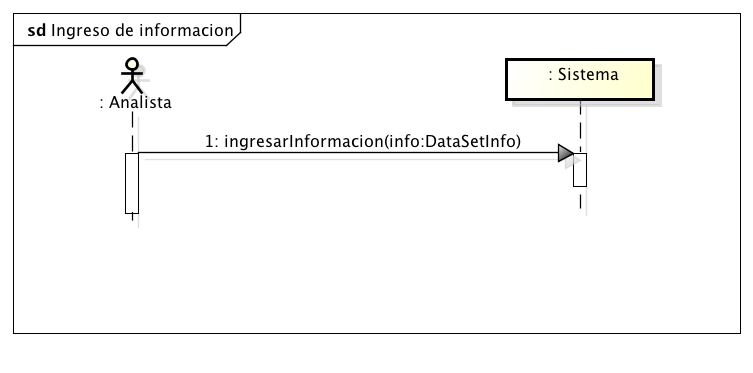
\includegraphics[width=5.7638in,height=2.8547in]{Analisisdelproblema-img/Analisisdelproblema-img007.png}
    Figura \stepcounter{Figura}{\theFigura} - caso de uso de ingreso de información
\end{figure}

\begin{figure}[h]
  \centering
    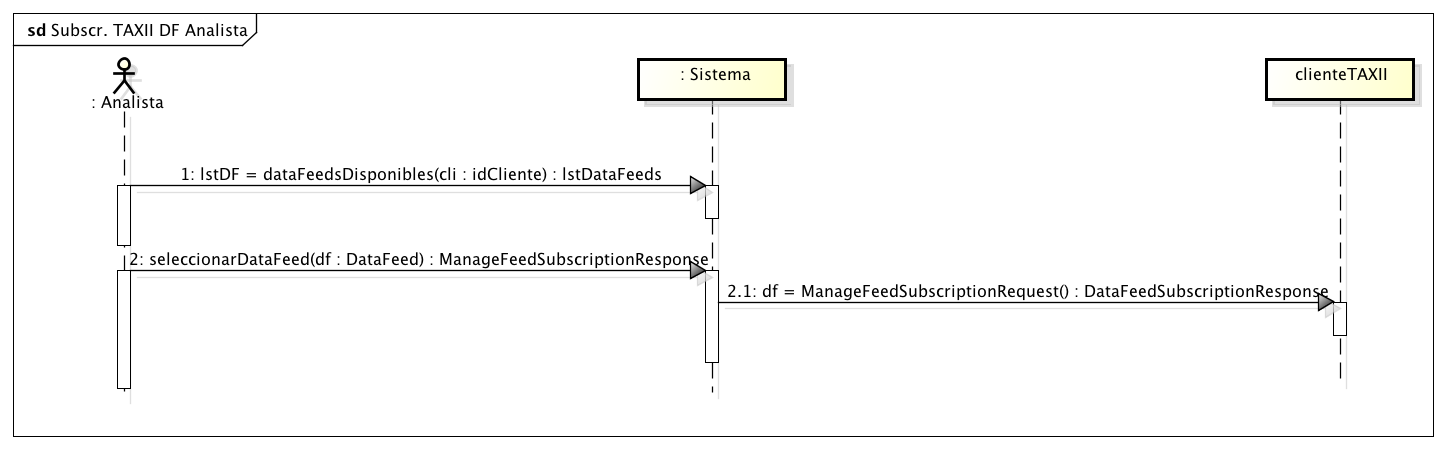
\includegraphics[width=5.7638in,height=1.8965in]{Analisisdelproblema-img/Analisisdelproblema-img008.png}
     Figura \stepcounter{Figura}{\theFigura} - Caso de uso subscribirse a un Data Feed
\end{figure}

\begin{figure}[h]
  \centering
    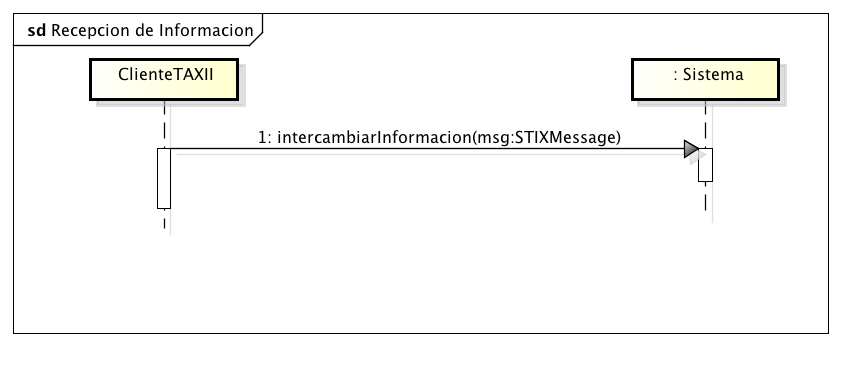
\includegraphics[width=5.7638in,height=2.5563in]{Analisisdelproblema-img/Analisisdelproblema-img009.png}
    Figura \stepcounter{Figura}{\theFigura} - Caso de uso de recepción de información
\end{figure}

\begin{figure}[h!]
    \centering
        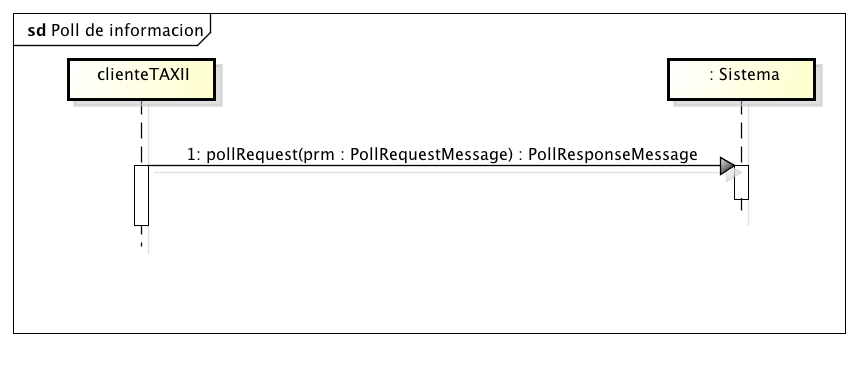
\includegraphics[width=5.7638in,height=2.5055in]{Analisisdelproblema-img/Analisisdelproblema-img010.png}
        Figura \stepcounter{Figura}{\theFigura} - Caso de uso poll de información
\end{figure}
\newpage
Para los casos de uso que son similares pero en los que cambia el sistema que hace el pedido no se presentan los diagramas.
\newpage
\subsection[Contratos]{Contratos}
\bigskip

\begin{flushleft}
\tablefirsthead{}
\tablehead{}
\tabletail{}
\tablelasttail{}
\begin{supertabular}{|m{1.0115598in}|m{4.7441597in}|}
\hline
Nombre &
ingresarInformacion\\\hline
Operación &
ingresarInformacion(info:DataSetInfo)\\\hline
Entrada &
Info representa los datos de la información que se desea ingresar al sistema.\\\hline
Salida &
No aplica\\\hline
Descripción &
Ingresa al sistema la información que el analista desee agregar.\\\hline
\end{supertabular}
\end{flushleft}

\bigskip

\begin{flushleft}
\tablefirsthead{}
\tablehead{}
\tabletail{}
\tablelasttail{}
\begin{supertabular}{|m{1.0115598in}|m{4.7441597in}|}
\hline
Nombre &
dataFeedsDisponibles\\\hline
Operación &
lstDF := dataFeedsDisponibles(cli : idCliente) : lstDataFeed\\\hline
Entrada &
Se pasa como parámetro el id del cliente en el sistema.\\\hline
Salida &
Se retorna una lista de los DataFeeds en dicho sistema.\\\hline
Descripción &
La operación retorna una lista con los DataFeeds existentes en el cliente pasado como parámetro.\\\hline
\end{supertabular}
\end{flushleft}

\bigskip

\begin{flushleft}
\tablefirsthead{}
\tablehead{}
\tabletail{}
\tablelasttail{}
\begin{supertabular}{|m{1.0115598in}|m{4.7441597in}|}
\hline
Nombre &
seleccionarDataFeed\\\hline
Operación &
seleccionarDataFeed(df : DataFeed) : msg\\\hline
Entrada &
El parámetro df representa un DataFeed en un cliente TAXII.\\\hline
Salida &
Se retorna un mensaje de éxito o error.\\\hline
Descripción &
La operación trata de suscribir el sistema a un nuevo TAXII Data Feed en un cliente TAXII.\\\hline
\end{supertabular}
\end{flushleft}

\bigskip
\newpage
\begin{flushleft}
\tablefirsthead{}
\tablehead{}
\tabletail{}
\tablelasttail{}
\begin{supertabular}{|m{1.0115598in}|m{4.7441597in}|}
\hline
Nombre &
ManageFeedSubscriptionRequest\\\hline
Operación &
Df := ManageFeedSubscriptionRequest() : DataFeedSubscriptionResponse\\\hline
Entrada &
~
\\\hline
Salida &
Se retorna un mensaje Feed Subscription Response Message con el resultado de la operación.\\\hline
Descripción &
La operación se lleva a acabo entre un cliente TAXII y el otro. El cliente trata de subscribirse en el otro para así poder intercambiar información.\\\hline
\end{supertabular}
\end{flushleft}

\bigskip

\begin{flushleft}
\tablefirsthead{}
\tablehead{}
\tabletail{}
\tablelasttail{}
\begin{supertabular}{|m{1.0115598in}|m{4.7441597in}|}
\hline
Nombre &
intercambiarInformacion\\\hline
Operación &
intercambiarInformacion(msg:STIXMessage)\\\hline
Entrada &
Se recibe como parámetro un mensaje STIX.\\\hline
Salida &
~
\\\hline
Descripción &
La operación envía al Inbox Service de otro cliente un mensaje STIX. Este incluye la información de seguridad a intercambiar.\\\hline
\end{supertabular}
\end{flushleft}

\bigskip

\begin{flushleft}
\tablefirsthead{}
\tablehead{}
\tabletail{}
\tablelasttail{}
\begin{supertabular}{|m{1.0115598in}|m{4.7441597in}|}
\hline
Nombre &
pollRequest\\\hline
Operación &
pollRequest(prm:PollRequestMessage) : pollResponseMessage\\\hline
Entrada &
Prm representa la información que se desea recibir del servidor.\\\hline
Salida &
Se retorna la información que se pidió por medio de prm.\\\hline
Descripción &
La operación retorna la información deseada, \ el prm es el que identifica la información en el servidor.\\\hline
\end{supertabular}
\end{flushleft}

\bigskip
\end{document}
